% \documentclass[handout]{beamer}
\documentclass{beamer}

\mode<presentation>
{
  \usetheme{ANLBlue}
  % \usefonttheme[onlymath]{serif}
  % \usetheme{Singapore}
  % \usetheme{Warsaw}
  % \usetheme{Malmoe}
  % \useinnertheme{circles}
  % \useoutertheme{infolines}
  % \useinnertheme{rounded}

  \setbeamercovered{transparent=20}
}

\usepackage[english]{babel}
\usepackage[latin1]{inputenc}
\usepackage{alltt,listings,multirow,ulem,siunitx}
\usepackage[absolute,overlay]{textpos}
\TPGrid{1}{1}
\usepackage{pdfpages}
\usepackage{ulem}
\usepackage{multimedia}
\usepackage{multicol}
\newcommand\hmmax{0}
\newcommand\bmmax{0}
\usepackage{bm}
\usepackage{comment}
\usepackage{subcaption}

% font definitions, try \usepackage{ae} instead of the following
% three lines if you don't like this look
\usepackage{mathptmx}
\usepackage[scaled=.90]{helvet}
% \usepackage{courier}
\usepackage[T1]{fontenc}
\usepackage{tikz}
\usetikzlibrary{decorations.pathreplacing}
\usetikzlibrary{shadows,arrows,shapes.misc,shapes.arrows,shapes.multipart,arrows,decorations.pathmorphing,backgrounds,positioning,fit,petri,calc,shadows,chains,matrix}

\newcommand\vvec{\bm v}
\newcommand\bvec{\bm b}
\newcommand\bxk{\bvec_0 \times \kappa_0 \cdot \nabla}
\newcommand\delp{\nabla_\perp}

% \usepackage{pgfpages}
% \pgfpagesuselayout{4 on 1}[a4paper,landscape,border shrink=5mm]

\usepackage{JedMacros}

\newcommand{\timeR}{t_{\mathrm{R}}}
\newcommand{\timeW}{t_{\mathrm{W}}}
\newcommand{\mglevel}{\ensuremath{\ell}}
\newcommand{\mglevelcp}{\ensuremath{\mglevel_{\mathrm{cp}}}}
\newcommand{\mglevelcoarse}{\ensuremath{\mglevel_{\mathrm{coarse}}}}
\newcommand{\mglevelfine}{\ensuremath{\mglevel_{\mathrm{fine}}}}

%solution and residual
\newcommand{\vx}{\ensuremath{x}}
\newcommand{\vc}{\ensuremath{\hat{x}}}
\newcommand{\vr}{\ensuremath{r}}
\newcommand{\vb}{\ensuremath{b}}

%operators
\newcommand{\vA}{\ensuremath{A}}
\newcommand{\vP}{\ensuremath{I_H^h}}
\newcommand{\vS}{\ensuremath{S}}
\newcommand{\vR}{\ensuremath{I_h^H}}
\newcommand{\vI}{\ensuremath{\hat I_h^H}}
\newcommand{\vV}{\ensuremath{\mathbf{V}}}
\newcommand{\vF}{\ensuremath{F}}
\newcommand{\vtau}{\ensuremath{\mathbf{\tau}}}


\title{How can we quantify \\ performance versatility?}
\author{{\bf Jed Brown} \texttt{jedbrown@mcs.anl.gov} (ANL and CU Boulder)}

% Real applications are often constrained by factors such as external
% requirements for time-to-solution, a need to fit within some level of
% memory, or to accommodate workflow demands involving human decisions,
% provenance, proprietary software, or the like.  Consequently, the region
% of multi-dimensional configuration space that an application cares about
% may be disjoint from the single point or path chosen by authors when
% promoting their new algorithm or machine.  Different authors are likely
% to choose different configurations, leading to results that are not very
% useful to applications.  Drawing on experience and performance data
% obtained while developing the HPGMG benchmark (https://hpgmg.org) and
% working with PETSc applications, we discuss issues and methods for
% collecting and presenting performance data to express versatility and
% improve relevance to applications.

% - Use the \inst command only if there are several affiliations.
% - Keep it simple, no one is interested in your street address.
% \institute
% {
%   Mathematics and Computer Science Division \\ Argonne National Laboratory
% }

\date{JointLab, Chicago, 2014-11-24 \\[1em]
{\small This talk: \url{http://59A2.org/files/20141124-Versatility.pdf}}}

% This is only inserted into the PDF information catalog. Can be left
% out.
\subject{Talks}


% If you have a file called "university-logo-filename.xxx", where xxx
% is a graphic format that can be processed by latex or pdflatex,
% resp., then you can add a logo as follows:

% \pgfdeclareimage[height=0.5cm]{university-logo}{university-logo-filename}
% \logo{\pgfuseimage{university-logo}}



% Delete this, if you do not want the table of contents to pop up at
% the beginning of each subsection:
% \AtBeginSubsection[]
% {
% \begin{frame}<beamer>
%   \frametitle{Outline}
%   \tableofcontents[currentsection,currentsubsection]
% \end{frame}
% }

% \AtBeginSection[]
% {
%   \begin{frame}<beamer>
%     \frametitle{Outline}
%     \tableofcontents[currentsection]
%   \end{frame}
% }

% If you wish to uncover everything in a step-wise fashion, uncomment
% the following command:

% \beamerdefaultoverlayspecification{<+->}

\begin{document}
\lstset{language=C}
\normalem

\begin{frame}
  \titlepage
\end{frame}

\begin{frame}{Why do we need an exascale computer?}
  \begin{itemize}
  \item Science \& engineering demands
    \begin{itemize}
    \item Model fidelity: resolution, multi-scale, coupling
    \item Inversion/data assimilation
    \item Optimization, control
    \item Quantify uncertainty, risk-aware decisions
    \item Sequence of forward simulations, each needing more time steps
    \end{itemize}
  \item External requirements on time-to-solution
    \begin{itemize}
    \item Policy: 5 SYPD for climate model to inform IPCC
    \item Weather: 250x faster than real-time
    \item Supply chain dynamics, manufacturing
    \item Field studies, disaster response
    \item Transient simulation is not weak scaling
    \end{itemize}
  \item ``weak scaling'' [\ldots] will increasingly give way to ``strong scaling''\\
    {\small [The International Exascale Software Project Roadmap, 2011]}
  \end{itemize}
\end{frame}

\begin{frame}{Is the tail wagging the dog?}
  \begin{itemize}
  \item Creative thinking about science/engineering problems
    \begin{itemize}
    \item Guide software and hardware choices
    \item Scientist: ``your code doesn't scale''
    \item Center: ``your machine is inappropriate for my application''
    \end{itemize}
  \item Find corners of ``science'' that can use the machines
    \begin{itemize}
    \item Incentivize solving problems hardware is good at
      \begin{itemize}
      \item funding, allocations
      \item ``if your code doesn't run on machine X, I'm not paying''
      \end{itemize}
    \item ``The easiest way to make software scalable is to make it sequentially inefficient'' -- Gropp (1999)
      \begin{itemize}
      \item Suboptimal modeling/algorithms are subtle inefficiency
      \end{itemize}
    \item Fragmenting high-end from low-end, no middle
    \item Opportunity in advancing low-end to medium scale
    \end{itemize}
  \end{itemize}
\end{frame}

\begin{frame}{Versatility}
  \begin{itemize}
  \item Solve problems of maximum science/engineering interest
  \item At practical accuracy
  \item With desired turn-around time
  \item On available hardware
  \item Using modular, extensible software
  \item Reliably, debuggable
  \item Automate everything
  \end{itemize}
\end{frame}

\begin{frame}{Why a new benchmark?}
  \begin{block}{Goodhart's Law}
    When a measure becomes a target, it ceases to be a good measure.
  \end{block}
  \begin{itemize}
  \item But surely we can do better than HPL
    \begin{itemize}
    \item Every feature stressed by benchmark should be {\bf necessary} for an important application
    \item Good performance on the benchmark should be {\bf sufficient} for good performance on most applications
    \end{itemize}
  \end{itemize}
\end{frame}

\begin{frame}{HPGMG: a new benchmarking proposal}
  \begin{itemize}
  \item \url{https://hpgmg.org}, hpgmg-forum@hpgmg.org mailing list
  \item Mark Adams, Sam Williams (finite-volume), Jed Brown (finite-element), John Shalf, Brian Van Straalen, Erich Strohmeier, Rich Vuduc
  \item Building momentum, BoF at SC14
  \item Implementations
    \begin{description}
    \item[Finite Volume] memory bandwidth intensive, simple data dependencies
    \item[Finite Element] compute- and cache-intensive, vectorizes, overlapping writes
    \end{description}
  \item Full multigrid, well-defined, scale-free problem
  \item Best-known algorithms, no ``fat'' left to trim
  \item Representative of structure-exploiting algorithms
  \end{itemize}
\end{frame}

\begin{frame}{SuperMUC (FDR 10, E5-2680)}
  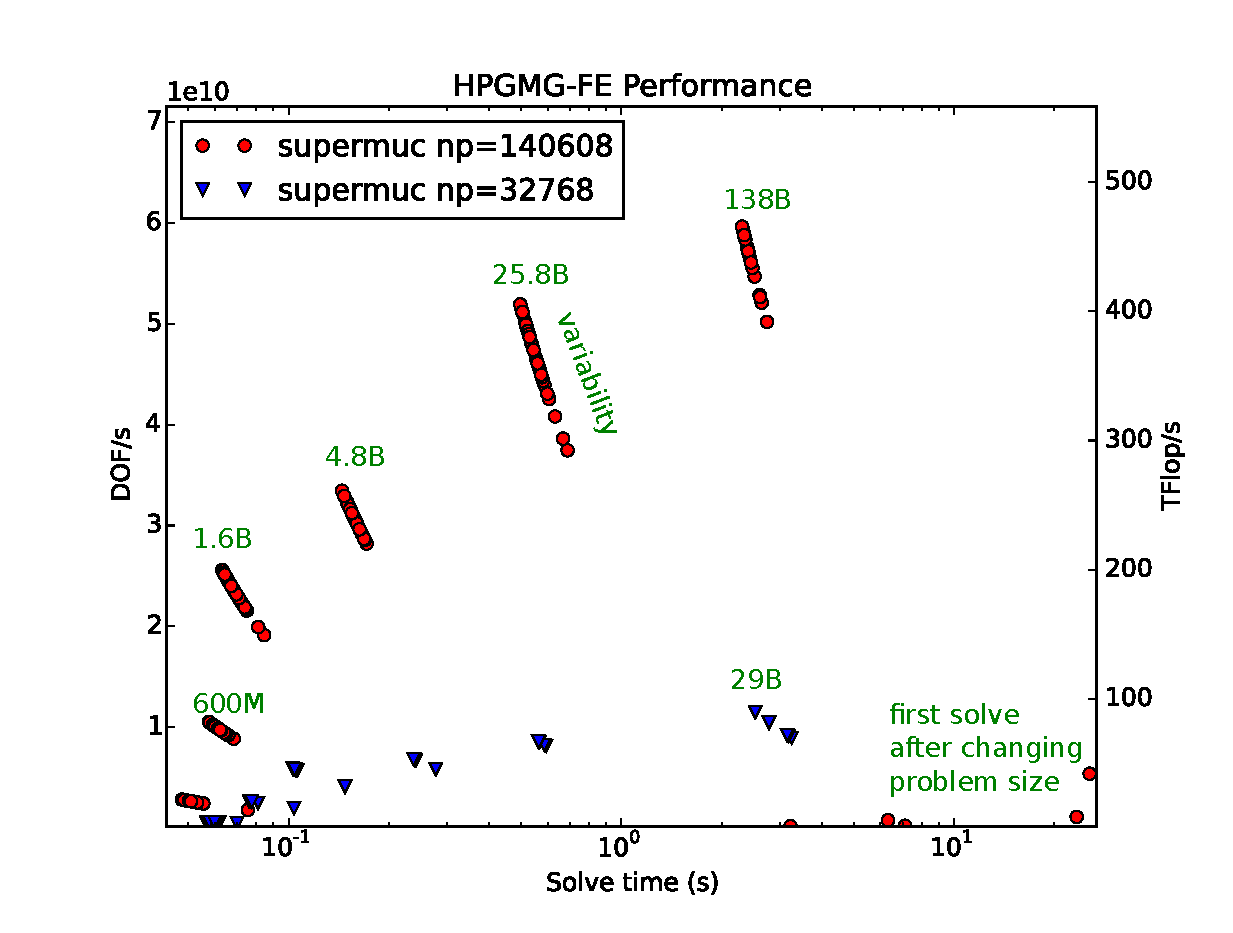
\includegraphics[width=\textwidth]{figures/hpgmg/range-supermuc-ann.eps}
\end{frame}

\begin{frame}{Edison (Aries, E5-2695v2)}
  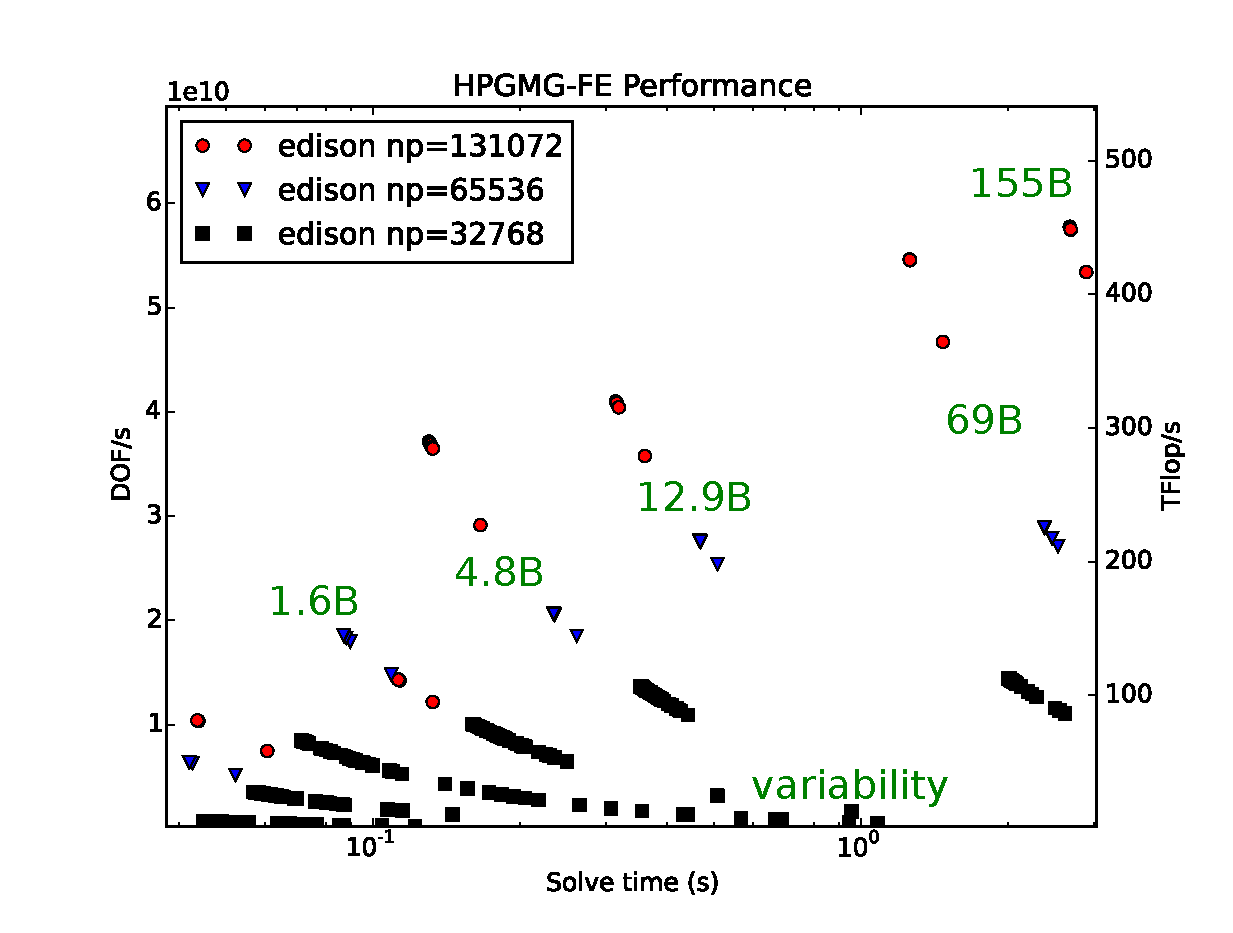
\includegraphics[width=\textwidth]{figures/hpgmg/range-edison-ann.eps}
\end{frame}

\begin{frame}{Edison, SuperMUC, Titan}
  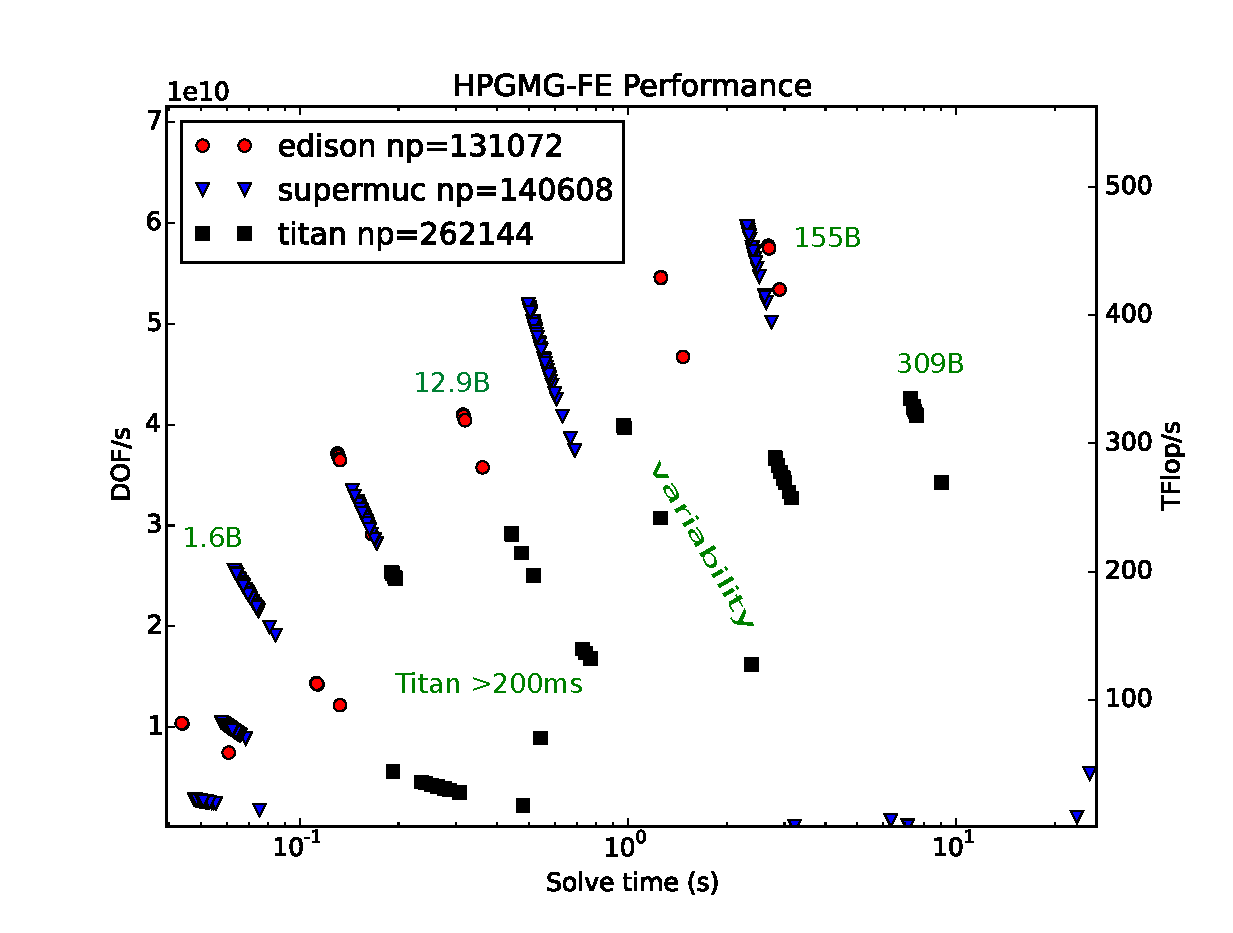
\includegraphics[width=\textwidth]{figures/hpgmg/range-edison-supermuc-titan-ann.eps}
\end{frame}

% \begin{frame}{Kiviat diagrams}
%   \begin{center}
%     \includegraphics[width=\textwidth]{figures/hpgmg-kiviat-20140606.png}
%   \end{center}
%   \begin{itemize}
%   \item c/o Ian Karlin and Bert Still (LLNL)
%   \end{itemize}
% \end{frame}

\begin{frame}{HPGMG distinguishes networks at 1M dofs/core}
  \begin{center}
    \includegraphics[width=0.6\textwidth]{figures/hpgmg-fv-20140515-dof.png}
  \end{center}
  \begin{itemize}
  \item Peregrine and Edison have identical node architecture
  \item Peregrine has 5:1 tapered IB, Edison has Aries dragonfly topology
  \end{itemize}
\end{frame}

\begin{frame}{MIC communication bottlenecks on Stampede}
  \begin{center}
    \includegraphics[width=\textwidth]{figures/hpgmg/fv-mic-mpi.png}
  \end{center}
\end{frame}

\begin{frame}{Hardware Arithmetic Intensity}
  \begin{tabular}{lc}
    \toprule
    Operation                         & Arithmetic Intensity (flops/B) \\
    \midrule
    Sparse matrix-vector product      & 1/6                  \\
    Dense matrix-vector product       & 1/4                  \\
    Unassembled matrix-vector product & $\approx 8$          \\
    High-order residual evaluation    & $> 5$                \\
    \bottomrule
  \end{tabular}

  \bigskip

  \begin{tabular}{lrrr}
    \toprule
    Processor & BW (GB/s) & Peak (GF/s) & Balanced AI (F/B) \\
    \midrule
    E5-2670 8-core      & 35   & 166  & 4.7 \\
    Magny Cours 16-core & 49   & 281  & 5.7 \\
    Blue Gene/Q node    & 43   & 205  & 4.8 \\
    Tesla M2090         & 120  & 665  & 5.5 \\
    Kepler K20Xm        & 160 & 1310 & 8.2 \\ % http://www.elekslabs.com/2012/11/nvidia-tesla-k20-benchmark-facts.html
    Xeon Phi            & 150 & 1248 & 8.3 \\
    \bottomrule
  \end{tabular}
\end{frame}

\begin{frame}{How much parallelism out of how much cache?}
  \begin{tabular}{l rrrr rr}
    \toprule
    Processor & v width & threads & F/inst & latency & L1D & L1D/\#par \\
    \midrule
    Nehalem & 2 & 1 & 2 & 5 & 32 KiB & 1638 B \\
    Sandy Bridge & 4 & 2 & 2 & 5 & 32 KiB & 819 B \\
    Haswell & 4 & 2 & 4 & 5 & 32 KiB & 410 B \\
    BG/P & 2 & 1 & 2 & 6 & 32 KiB & 1365 B \\
    BG/Q & 4 & 4 & 2 & 6 & 32 KiB & 682 B \\
    KNC & 8 & 4 & 4 & 5 & 32 KiB & 205 B \\
    Tesla K20 & 32 & * & 2 & 10 & 64 KiB & 102 B \\
    \bottomrule
  \end{tabular}
  \begin{itemize}
  \item Most ``fast'' algorithms do about $O(n)$ flops on $n$ data
  \item DGEMM and friends do $O(n^{3/2})$ flops on $n$ data
  \item Exploitable parallelism limited by cache and register load/store
  \item L2/L3 performance highly variable between architectures
  \end{itemize}
\end{frame}

\begin{frame}{Where we are now: $QR$ factorization with MKL on MIC}
  \begin{figure}
    \centering
    \includegraphics[width=\textwidth]{figures/hardware/MKL-dgeqrf-MIC-201411.png}
  \end{figure}
  \begin{itemize}
  \item Figure compares two CPU sockets (230W TDP) to one MIC (300W TDP plus host)
  \item Performance/Watt only breaks even at largest problem sizes
  \item Haswell-EP doubles performance within same power envelope
  \item $10^4 \times 10^4$ matrix takes 667 GFlops: about 2 seconds
  \item This is an $O(n^{3/2})$ operation on $n$ data
  \item MIC cannot strong scale, no more energy efficient/cost effective
  \item ``hard to program'' versus ``architecture ill-suited for problem''?
  \end{itemize}
\end{frame}

\begin{frame}{Outlook}
  \begin{itemize}
  \item How can we measure versatility?
    \begin{itemize}
    \item Opportunity cost of avoiding problems that ``don't scale''
    \end{itemize}
  \item What is the impact of performance variability?
    \begin{itemize}
    \item Allocation budgeting, coupling, load balancing
    \end{itemize}
  \item We should strive to put ourselves out of business
  \end{itemize}
\end{frame}

\end{document}
